% MA211 - Lecture 2
\documentclass[pdftex, xcolor=pdftex, dvipsnames, handout]{beamer}

\usetheme{MA211}
\usepackage{thumbpdf}
\usepackage{wasysym}
%\usepackage{ucs}
\usepackage[utf8]{inputenc}
\usepackage{pgf,pgfarrows,pgfnodes,pgfautomata,pgfheaps,pgfshade}
\usepackage{verbatim}

\usepackage{eurosym}
\usepackage{euler}

\usepackage{calc}               % Simple computations with LaTeX variables
%\usepackage[hang]{caption2}     % Improved captions

\usepackage{graphicx}           % Standard graphics package

\usepackage{amsmath, amsthm, amssymb}


\newcommand{\fquad}{\mbox{\qquad}}
\newcommand{\bull}{$\bullet$ }

\newcommand {\I} {\mathcal I}
\newcommand {\calI} {\mathcal I}
\def\disint{\displaystyle\int}

\DeclareMathOperator{\D}{d}
\newcommand{\dydx}{\frac{\D y}{\D x}}

%\definecolor{gray}{rgb}{0.69, 0.69, 0.69} \newcommand{\gray}[1]{\textcolor{gray}{#1}}
\definecolor{dogreen}{rgb}{0.33, 0.42, 0.18} \newcommand{\dogreen}[1]{\textcolor{dogreen}{#1}}
\definecolor{maroon}{rgb}{.5,0.2,0.2}\newcommand{\maroon}[1]{\textcolor{maroon}{#1}}
\definecolor{greena}{rgb}{.1,0.581,0.1}\newcommand{\greena}[1]{\textcolor{greena}{#1}}

\definecolor{blue4}{rgb}{0,0,.545}
\newcommand{\Blue}[1]{\textcolor{blue}{#1}}
\newcommand{\Red}[1]{\textcolor{red}{#1}}
\definecolor{pink}{rgb}{1.,0.75,0.8}
\definecolor{darkred}{rgb}{0.5,0.0,0.0}
\definecolor{darkgreen}{rgb}{0,0.3,0.3}
\definecolor{purple}{rgb}{0,0.3,0.3}
\definecolor{darkblue}{rgb}{0.0, 0.0, .5}
\definecolor{dpurple}{rgb}{.3,.0,.3}
\newcommand{\Green}[1]{\textcolor{darkgreen}{#1}}
\newcommand{\DRed}[1]{\textcolor{darkred}{#1}}
\newcommand{\DBlue}[1]{\textcolor{darkblue}{#1}}
\newcommand{\Purple}[1]{\textcolor{dpurple}{#1}}
\newcommand{\Emph}[1]{\textcolor{darkred}{\textbf{\it #1}}}
\newcommand{\remph}[1]{\textcolor{darkred}{\textbf{\emph{#1}}}}
\newcommand{\bemph}[1]{\textcolor{darkblue}{\textbf{\emph{#1}}}}
\newcommand{\gemph}[1]{\textcolor{darkgreen}{\textbf{\emph{#1}}}}
\newcommand{\Bf}[1]{\textcolor{darkblue}{\textbf{#1}}}
\newcommand{\Gf}[1]{\textcolor{darkgreen}{\textbf{#1}}}
\newcommand{\Rf}[1]{\textcolor{red}{\textbf{#1}}}
\newcommand{\Rmf}[1]{\textcolor{red}{\mathbf{#1}}}

\newcommand{\Conj}[1]{\overline{#1}}

\newcommand{\code}[1]{\textcolor{darkblue}{\texttt{\textbf{#1}}}}
\newcommand{\icode}[1]{{\blue\texttt{\textbf{\emph{#1}}}}}
\newcommand{\gcode}[1]{{\Green{\texttt{\textbf{\emph{#1}}}}}}
\newcommand{\out}[1]{\texttt{\emph{\textbf{\Green{#1}}}}}





\newenvironment{vminipage}%
{\begin{Sbox}\begin{minipage}\begin{small}\begin{verbatim}}%
{\end{verbatim}\end{small}\end{minipage}\end{Sbox}\fbox{\TheSbox}}

\newenvironment{nminipage}%
{\begin{Sbox}\begin{minipage}}%
{\end{minipage}\end{Sbox}\fbox{\TheSbox}}


\let\Arg\relax\DeclareMathOperator{\Arg}{\mathtt{Arg}}
\let\Arg\relax\DeclareMathOperator{\e}{\mathtt{e}}

\newcommand {\AND} {\wedge}
\newcommand {\OR} {\vee}
\newcommand {\NOT} {\neg}
\newcommand {\IMPLIES} {\rightarrow}
%\newcommand {\IFF} {\leftrightarrow}
\renewcommand {\iff} {\Leftrightarrow}
\newcommand {\NAND} {\uparrow}
\newcommand {\NOR} {\downarrow}
\newcommand {\XOR} {\otimes}

\newenvironment{citemize}% Colour items
{\begin{description}}%
{\end{description}}

\newcommand {\maroonitem}{\item[\maroon{$\bullet$}]}

\newcommand {\gitem} {\item {\includegraphics[width=.4cm,angle=-10]{img/green-bullet-on-white.ps}}}
\newcommand {\ritem} {\item {\includegraphics[width=.4cm,angle=-10]{img/red-bullet-on-white.ps}}}
\newcommand {\yitem} {\item {\includegraphics[width=.4cm,angle=-10]{img/yellow-bullet-on-white.ps}}}
\newcommand {\bitem} {\item {\includegraphics[width=.4cm,angle=-10]{img/blue-bullet-on-white.ps}}}

\newcommand {\greenitem} {\item {\includegraphics[width=.4cm,angle=-10]{img/green-bullet-on-white.ps}}}
\newcommand {\reditem} {\item {\includegraphics[width=.4cm,angle=-10]{img/red-bullet-on-white.ps}}}
\newcommand {\yellowitem} {\item {\includegraphics[width=.4cm,angle=-10]{img/yellow-bullet-on-white.ps}}}
\newcommand {\blueitem} {\item {\includegraphics[width=.4cm,angle=-10]{img/blue-bullet-on-white.ps}}}

\newcommand {\eq}[1]%
  {$\DBlue{#1}$}
\newcommand {\eqd}[1]%
  {$\displaystyle\DBlue{#1}$}
%\newcommand{\eq}[1]{\boldmath \DBlue{$#1$}}


\newcommand {\csf}{\centerslidesfalse}
\newcommand {\cst}{\centerslidestrue}

\newcommand {\vecii}[2] {   \big(\begin{smallmatrix} #1 \\ #2 \end{smallmatrix}\big)}
\newcommand{\atwo}[2]{\left(\!\!\begin{array}{c} #1 \\ #2 \end{array}\!\!\right)}


\newcommand{\C}{\mathbb{C}}
\newcommand{\Q}{\mathbb{Q}}
\newcommand{\R}{\mathbb{R}}
\newcommand{\N}{\mathbb{N}}
\newcommand{\Z}{\protect\mathbb{Z}}  % protect for index.
\newcommand {\Rs}{ \mathbb{R}}
\newcommand {\Cs}{ \mathbb{C}}
\newcommand {\Rnn}{ \mathbb{R}^{n \times n}}
\newcommand {\Rn}{ \mathbb{R}^{n}}


\newcommand{\mblock}{%
\setbeamercolor*{block title}{bg=maroon,fg=white}
\setbeamercolor*{block body}{bg=white,fg=maroon}
}%

\newcommand{\bblock}{%
\setbeamercolor*{block title}{bg=Steel,fg=white}
\setbeamercolor*{block body}{bg=Mylightgray,fg=Steel}
}%

\newcommand{\gblock}{%
\setbeamercolor*{block title}{bg=Green,fg=white}
\setbeamercolor*{block body}{bg=Mylightgray,fg=darkgreen}
}%


\newcommand{\rblock}{%
\setbeamercolor*{block title}{bg=Red,fg=white}
\setbeamercolor*{block body}{bg=white,fg=Black}
}%


\newcommand{\TakeNotes}{
\includegraphics[width=2cm]{TakeNote}}



\def\eps{\varepsilon}
\newcommand {\del}[2]{ {\frac{\partial #1}{\partial #2}}}
\newcommand {\x}[1]{x^{[#1]}}
\newcommand {\delx}{ {\frac{\partial}{\partial x}}}
\newcommand {\delt}{ {\frac{\partial}{\partial t}}}
\newcommand {\dely}{ {\frac{\partial}{\partial y}}}
\newcommand {\ith}{{(i)}}
\renewcommand {\vec}[1]{ {\boldsymbol{#1}}}
\newcommand {\Oh} {\mathcal O}
\newcommand {\Err} {\mathcal E}
%\newcommand {\th} {\mathrm{th}}
\DeclareMathOperator{\fl}{fl}
\DeclareMathOperator{\sign}{sign}
\DeclareMathOperator{\Cond}{Cond} 
\DeclareMathOperator{\cond}{cond}
\DeclareMathOperator{\diag}{diag} 
\DeclareMathOperator{\sym}{sym} 
\DeclareMathOperator{\Trace}{Trace}
\DeclareMathOperator{\E}{e}

\newcommand {\Rsym}{{ \mathbb{R}^{n \times n}_\mathrm{sym}}}

\parskip .25cm


\theoremstyle{definition}
\newtheorem{exercise}{Exercise}[section]
\newtheorem{method}{Method}[section]



\subtitle{MA211 : Calculus, Part 1}
\title{Lecture 2: Sets and Functions}

\author{Dr Niall Madden (Mathematics, NUI Galway)}

\date{\Large Wednesday, 10 September 2008}


\begin{document}


\frame{

\begin{block}{}
\begin{center}
{\large \insertsubtitle}

\vspace{.1cm}

\begin{Large}
\textbf{\inserttitle}
\end{Large}

\vspace{.15cm}

{\footnotesize \insertauthor}

\vspace{.4cm}

{ {\insertdate}}
\end{center}
\end{block}


\vspace{-0.25cm}
\begin{center}
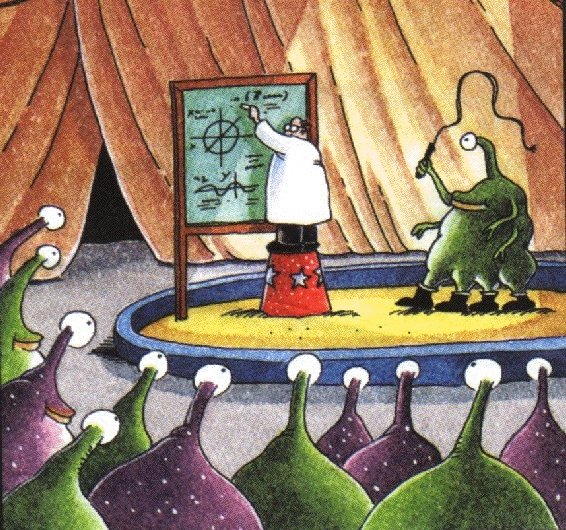
\includegraphics[height=4cm]{images/EventCalculus}
\end{center}
}



%\section{Outline}
\frame{
  \frametitle{Outline}
 \tableofcontents



}


\frame{

\frametitle{Welcome to MA211}
(\emph{The next 13 frames contain a short summary of the information
  provided at Monday's Lecture})

This is Semester 1 of the Second Year Calculus course.

~

\begin{columns}[c]
\column{4cm}
\Bf{Lecturer:}\\ \textbf{Dr Niall Madden,\\ Dep of Mathematics}, \\
Room 103,\\
\href{http://www.maths.nuigalway.ie/~niall/NUIGalwayMapRiverside.jpg}{Riverside
  Terrapin},\\ Distillery Road.\\ 

{\small \code{\href{mailto:Niall.Madden@NUIGalway.ie}{Niall.Madden@NUIGalway.ie}}}\\
Phone (091 49) 3803.

\column{5.5cm}
\begin{center}
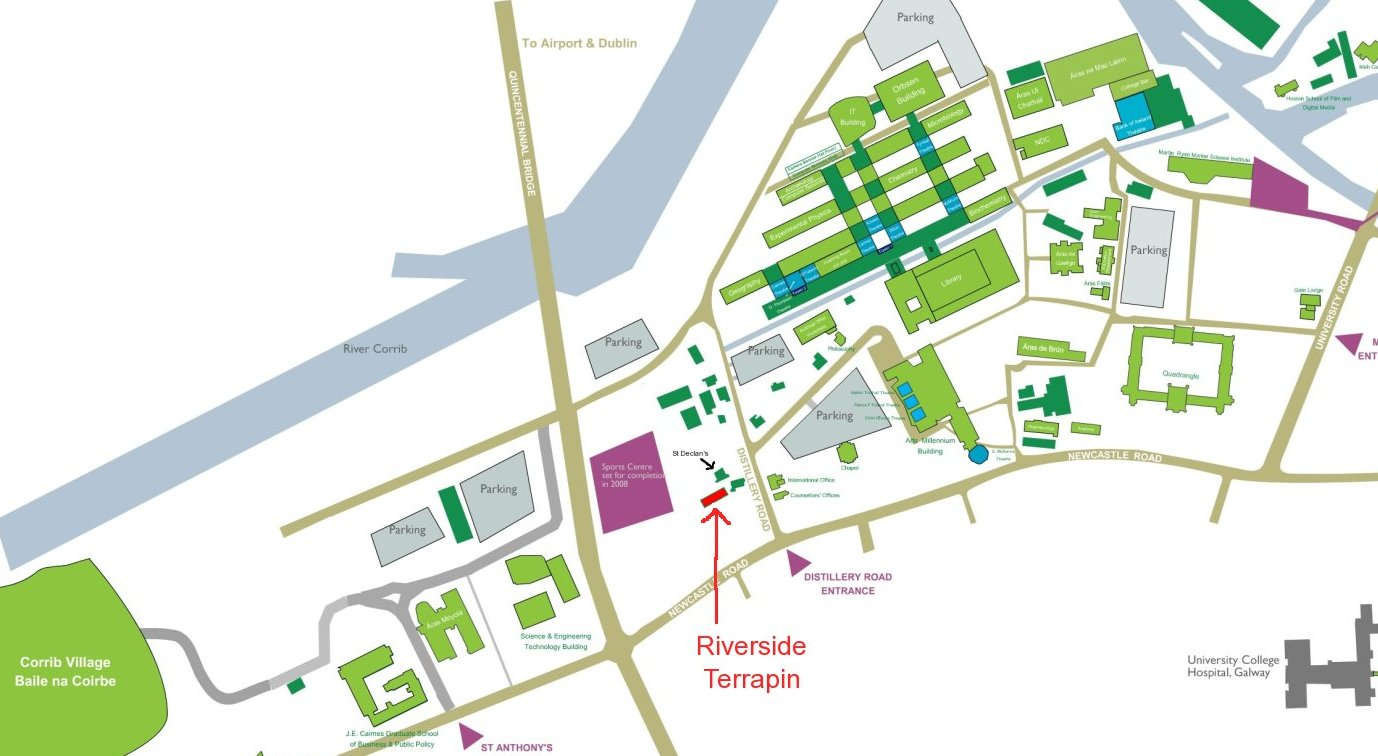
\includegraphics[width=0.95\textwidth]{NUIGalwayMapRiverside_small}
\end{center}

\end{columns}
}


\frame{
\frametitle{Schedule}

\begin{description}
\item[Lectures:] Monday and Wednesday, 11-12 in the Cairnes Lecture Theatre.

\item[Tutorials:] \Emph{Provisional Schedule}
\begin{itemize}
\item Tuesdays 3-4, AC202
\item Wednesdays 5-6 QA003 Physiology
\item Thursdays 6-7  IT205
\end{itemize}

Tutorials will being during week 3.
\end{description}
}



\frame{

\frametitle{Website}
\begin{center} 

\includegraphics[width=6cm]{images/Bblogo_Gateway_Large}
\end{center}

The on-line resources for this course are on
\href{http://BlackBoard.NUIGalway.ie}{\code{http://BlackBoard.NUIGalway.ie}}.

There you'll find various pieces of information, including these
notes.

It may take a week or two for everyone to have access to BlackBoard. 
In the short term, we'll also use
\href{http://www.maths.NUIGalway.ie/MA211}{\code{http://www.maths.NUIGalway.ie/MA211}}.


}


\frame{
\frametitle{Lecture Notes}

\begin{center}

\includegraphics[width=2cm]{TakeNote}
\end{center}

A \Bf{summary of each lecture} will be posted to the site  no later
than 9.30 on the day of the lecture. 

\begin{center}
\Emph{Print these out and bring them with you to lectures.}
\end{center}

You will then annotate these notes during the class.

}


\frame{

\frametitle{Topics}
The key topics in \Bf{MA211} are (but  not in order)
\begin{enumerate}[<+->]
\item Sets and functions.

\item  Methods of integration: substitution, integration by parts,
  partial fractions, reduction formulae. 

\item  Improper integrals (as limits of finite integrals).

\item Differential equations: linear equations with constant
  coefficients, first order homogeneous equations, boundary value
  problems, etc.

\end{enumerate}

}


\frame{
\frametitle{Mathematical Preliminaries}

\begin{columns}[c]
\column{0.45\textwidth}

Anyone who can remember their first year calculus should be able for
this course.  

~

Where we make particular use of topics from 1st year, I will try to remind
you and give you a reference for a text-book.

~

If I don't, \alert{please ask!}

\column{0.55\textwidth}
\begin{center}
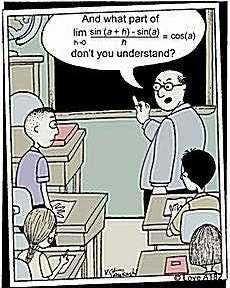
\includegraphics[width=5.5cm]{images/WhatPart}
\end{center}
\end{columns}


 
}

\frame{
\frametitle{Text book}


There is no required textbook for this course, but two are
particularly recommended:
\begin{enumerate}[<+->]
\item Stewart: \Emph{Calculus} and \Emph{Calculus: early
    transcendentals}. There are copies in the library, particularly of
   ``early transcendentals''.


\item Robert Adams, \Emph{Calculus: a short course, 3rd ED}, 515 ADA
%(Note: the library also has a few copies of the 5th ED. That one is
%less useful). 
There are 7 copies in the library.
\end{enumerate}

\pause
If you buy a copy of either of these, you will find it useful for MA211.

}
\frame{

\frametitle{Text book}

Also useful are:

\begin{enumerate}
\item Anton, \Emph{Calculus}, 515 ANT


\item Spiegel, \Emph{Advanced Calculus}, 515 SPI (12 copies in the library)
-- This is only for the 1st half of the course.
\end{enumerate}

In general: any book with \Emph{Calculus} in the title and that covers 
\begin{itemize}[<+->]
\item Integration, including Improper Integrals
\item Transcendental functions, in particular exponential, logarithmic
  and hyperbolic functions.
\item Differential equations.
\end{itemize}

}


\frame{
\frametitle{Course assessment}

Your progress in, and commitment to, this  course will be assessed as
follows:

\begin{itemize}
\item 
\Bf{Homework Assignment:}
There will be exercises included in every
  lecture. These will be collected into a series a problem sets which
  will be posted separately to Blackboard.  

  Every 3 weeks (approximately) you will be required to submit
  \Emph{carefully written solutions} to  selected exercises. These
  will be graded and returned to you. The mark you get will count
  towards you final MA211  grade 

\item 
\Bf{Class Test:}
 There will be a 30 minute class test during Week  6.

\item  \Bf{End of Semester Exam:}
Worth \Bf{75\%} of the total grade for
  MA211.
\end{itemize}

}


\frame{

\frametitle{What is Calculus?}


 \textbf{Wikipedia:} 
\emph{Calculus (from Latin, "pebble" or "little stone") is a branch of mathematics that
  includes the study of limits, derivatives, integrals, and infinite
  series, and constitutes a major part of modern university
  education. 

Calculus has widespread applications in science and
  engineering and is used to solve complex and expansive problems for
  which algebra alone is insufficient. 

It builds on analytic geometry
  and mathematical analysis and includes two major branches,
  differential calculus and integral calculus, that are related by the
  fundamental theorem of calculus.
  }



}


\frame{

\frametitle{Exercises}

\begin{exercise}[1.1]

 Go to to the library. Find where they keep the calculus
  books. Choose any three. Find the section where they introduce the
  concept of a \Bf{limit} of a function at a point. Write down the
  \Emph{definition of a limit} they provide, \Emph{their explanation
    of what it means}, and \emph{One example}.

Rank the books in order of how useful you think they are.


\end{exercise}

\begin{exercise}[1.2]


 The study of what we call ``Calculus'' is said to have been
  started by \emph{Isaac Newton} and \emph{Gottfried  von
    Leibniz}.

Find out
  when and where they lived, and what their major mathematical
  discoveries were.

\end{exercise}

} 


\section{Short review of sets}


\frame{


A \Bf{set}, roughly speaking, is a collection of objects.
It the set is made up of, for example, \eq{a}, \eq{b} and \eq{c}, we
write the set as
\[
\{a,b,c\}
\]

\pause

We give the set a name. For example, call it \eq{S}, and write
\[
S=\{a,b,c\}
\]

}

\frame{
When talking about the set \eq{S}, we might say things like
\begin{itemize}
\item  ``\emph{\eq{a} is an element of \eq{S}}'', 
\item  ``\emph{\eq{a} is an member of \eq{S}}'', 
\item ``\emph{\eq{S} contains  \eq{a}}''.
  \end{itemize}
and we write \eq{a \in S}.


We call the set \eq{B} a \emph{subset} of \eq{A} if every element of
\eq{B} is also in \eq{A}. 

\begin{example}
 Let \eq{S=\{a,b,c\}} and \eq{T=\{a,c\}}, then \eq{T} is
a subset set of \eq{A}. We write \eq{T \subseteq S}.
\end{example}
}

\section{Sets of numbers}
\subsection{The Naturals: $\N$}

\frame{


The most fundamental or ``\Emph{natural}'' set of numbers is, well, 
the \Bf{Natural Numbers: $\N = \{1, 2, 3, \dots \}$}.
These are the ones we use for counting.

But we can't use the for solving even simple \Emph{linear} equations such as:
\emph{find  \eq{x} such that}
\[
 \DBlue{x + 2 =0}.
\]
The solution to this is \eq{x=-2} which is not a natural number. So we must
also use negative numbers...
}

\subsection{The Integers: $\Z$}
\frame{
The next most obvious set of numbers is the \Bf{Integers}
\[
 \Z = \{\dots, -3, -2, -1, 0, 1, 2, 3, \dots \}.
\footnote{We use the symbol $\Z$ because of the German word \Emph{Zahlen},
meaning Integer}
\]
Note that every natural number is also an integer. Mathematically, we write
this as \eq{\N \subset \Z}. In English we read this as ``\emph{the Natural numbers
are contained in the set of Integers}''.\footnote{Or ``\emph{The Natural numbers
is a subset of the Integers}''. Or ``\emph{The Integers is a superset of the
Naturals}''.}

}

\frame{
 

But even the Integers is not a big enough set to contain the solutions to
even very simple equations.  For example:
\emph{find  \eq{x} such that}
\[
 \DBlue{3 x - 2 =0}.
\]
The solution to this is \eq{x=2/3} which is not an integer. So we have to
include fractions...
}


\subsection{The Rationals: $\Q$}

\frame{
The next set of number we try is called the \Emph{Rationals}, denoted by the
symbol $\Q$~\footnote{$\Q$ stands for \Emph{Q}uotient} which is made up of
all the numbers are can be expressed as fractions.

More precisely:
\[ 
  \DBlue{ \Q = \{ \frac{p}{q} \mid p, q \in \Z, \, q \neq 0\}.}
\]
This means that a number is \Emph{rational} if can be written as the ratio of
two integers. 

Examples:
\begin{itemize}
\item \DBlue{$3 \frac{3}{7} = \frac{24}{7}$} is rational.
\item \DBlue{$2.14 = 107/50$} is rational
\item \DBlue{$\pi=3.141 592 653 589 79...$} is \emph{not} rational - it has
an infinite decimal expansion.
\end{itemize}
}

\frame{
A more pertinent example of numbers that are not rational are the
solutions to the equation
\[
 \DBlue{x^2 - 2 =0}.
\]
The solutions: $\DBlue{x=\sqrt{2}}$ and $\DBlue{x=-\sqrt{2}}$ are not rational.

\pause 

\begin{exercise}[2.1]
Show that \eq{\sqrt{2}} is \emph{not} a rational
number. That is, show that there is no pair on integers \eq{a} and \eq{b}
such that \eq{a} and \eq{b} have no common divisors and \eq{(a/b)^2 =2}.

\Green{Hint:}  See Proposition 2.6 in Smith's \Emph{Introductory Mathematics}.
\end{exercise}
}

\frame{
Note that all the Integers (and so too the Naturals) are contained in the
Rationals:
\[
 \DBlue{\N \subset \Z \subset \Q.}
\]
}

\subsection{Real Numbers: $\R$}
\frame{
The \Emph{real  numbers: $\R$}, are \Emph{limits of sequences} of
  rational numbers such as
\[
    \DBlue{\sqrt{2} = 1.\pause 4\pause 1\pause 4\pause 2\pause 1\pause 3\pause 5\pause 6\ldots},
\]
\pause 
\[
    %\frac{\pi}{4} &= 1 - \frac13 + \frac15 - \frac17 \pm \dots &
    \DBlue{e = \frac1{0!} \pause + \frac1{1!} \pause + \frac1{2!} \pause  + \frac1{3!}  + \dots}.
\]
\pause

\begin{block}{}
\Bf{$\R$} is set of  numbers system you have used most often, and it is
the one we are most concerned about in this course.

%It contains all the sets mentioned in the earlier slides
%\[
%\DBlue{\N \subset \Z \subset \Q \subset \R}.
%\]

\end{block}


\begin{exercise}[2.2]
 What sets are usually represented by the symbols 
\begin{large}\begin{center}
$\R$, $\N$,
  $\Z$, $\Q$ and $\C$?
\end{center}
\end{large}
For each one, determine which of the others it
  is a subset of.
\end{exercise}
}

\frame{

\gblock

\begin{block}{Some Notation}
When we want to refer to some subset  of the real numbers, we sometimes
write it as
\begin{itemize}
\item \eq{[a,b]} meaning all numbers \eq{x} such that \eq{a \leq x \leq b}.
\item  \eq{(a,b)} meaning all numbers \eq{x} such that \eq{a < x < b}.
\end{itemize}

\end{block}

\begin{example}

\begin{itemize}
\item All \eq{x} strictly between 3 and 4:

~

\item All \eq{x} less that \eq{-1} 

~

\item All \eq{x} greater than or equal to \eq{4} 

~

~
\end{itemize}

\end{example}


}


\section{A short review of functions}
\subsection{Domain and Codomain}
\frame{

The idea of a \Emph{function} is one of the key concepts in
mathematics.

\begin{definition}[Function]
Given two sets \eq{X} and \eq{Y}, a \Bf{function} \eq{f} from \eq{X}
to \eq{Y} is a rule of
correspondences that associates every element of \eq{X} with some
(single)  element of \eq{Y}. We write:
\[
f: X \rightarrow Y.
\]

\begin{itemize}
\item \eq{X} is called the \Bf{Domain} of \eq{f}, and 
\item \eq{Y} is called the
\Emph{Codomain}.
\end{itemize}


If \eq{x \in X} is mapped to \eq{y} in \eq{Y} then we write
\eq{f(x)=y}. \\\pause Can also  say 
``\emph{\eq{f} sends \eq{x} to  \eq{y}}'' 
or 
``\emph{\eq{x} is the image of \eq{y} (under \eq{f})''} .
 
\end{definition}


}

\subsection{Domain and Range}

\frame{

If \eq{f:A \rightarrow B} the subset of elements of \eq{B} that are
images of elements of \eq{A} is called \Emph{Range} of \eq{f}, or the
\Bf{Image} of \eq{f}.


\begin{definition}[Range]
\eq{y} is in the range of \eq{f:A \rightarrow B} if there is some
\eq{x \in A} such that \eq{f(x)=y}.
\end{definition}

\begin{center}
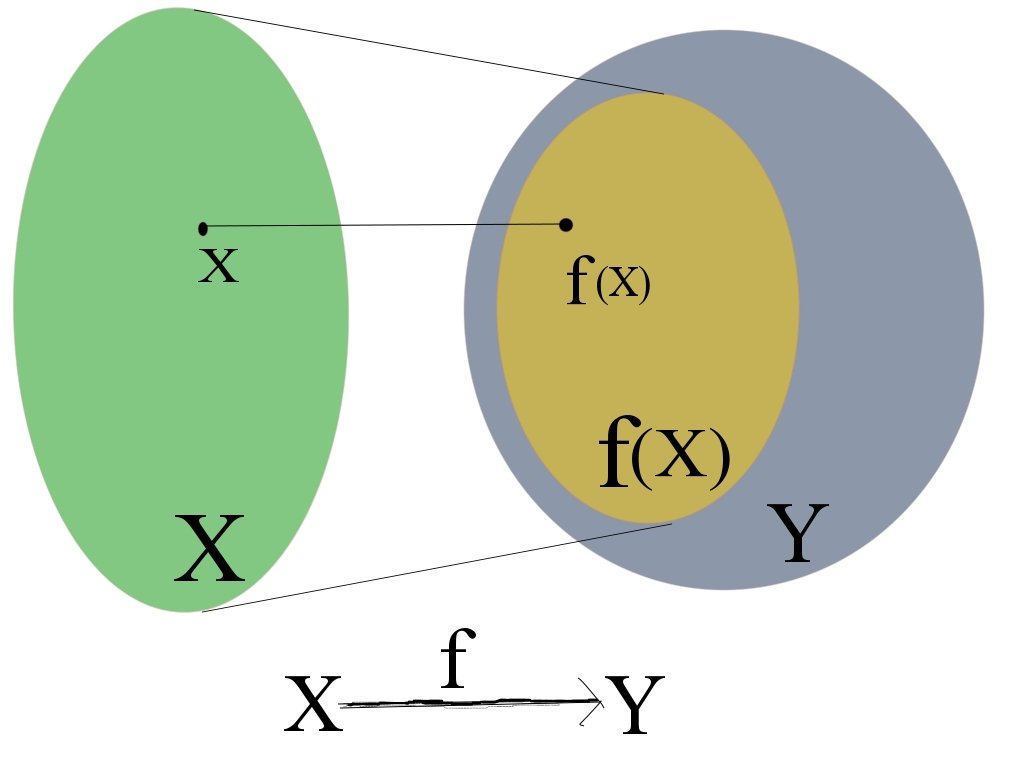
\includegraphics[width=5.5cm]{images/Codomain}
\end{center}

}

\frame{
In contrast with how it was presented in the last few slides, we most
often define a function simply by giving a formula for it, and leave
it to the reader to decide what the domain and range are.

\begin{example}[2.1]
Find the subsets of \eq{\R} that are the largest possible domain and
range for the function
\[ f(x) = x^2 + 1.\]
\end{example}


\vspace{2cm}

}

\frame{

\begin{example}[2.2]
What is the largest domain and range for the function \eq{ f(x) = \sqrt{x+2}}?
\end{example}

\vspace{4cm}

}

\frame{
\begin{example}[2.3]
Determine  the largest domain and range for the function 
\[  f(x) = \frac{1}{x^2-x}.\]
\end{example}

\vspace{4cm}

}

\frame{

\begin{exercise}[2.3]
For each of the following,  give the largest possible  subset of $\R$
that can be the domain and range:
\begin{enumerate}[(i)]
\item $f(t)=1/(1+t)$
\item $f(x) =\sqrt{9-x^2}$
\item $f(x) = \cos(x)$ 
\item $f(t) = \sin(5t-2)$.
\item \eqd{f(x) = 1 + \frac{1}{1-x^2}}.
\item $f(x) = e^x$.
\end{enumerate}
\end{exercise}
}

\section{Even and Odd functions}
\frame{

\begin{definition}
A function \eq{f} is called  \Bf{even} if \eq{f(-x)=f(x)}.

~

A function \eq{f} is called  \Bf{odd} if \eq{f(-x)=-f(x)}.

~

It is possible for a function to be nether \Bf{odd} nor \Emph{even}.
\end{definition}

\begin{example}
Show that the function 
\eqd{  f(x) = x^2 } is \Emph{even}.
\end{example}

\vspace{2cm}

}



\frame{

\begin{example}
Show that the function 
\eqd{f(x) = \frac{x^3 -x }{x^2+1}}
is \Bf{odd}.
\end{example}


\vspace{3cm}


}

\frame{

\begin{example}
Recall that the \Emph{absolute value function} is defined as 
\[
\|x\| = \begin{cases}
x & \text{ if } x \geq 0,\\
-x & \text{ if } x < 0.
\end{cases}
\]

\begin{enumerate}
\item Is the function $f(x) = |x|$ odd or even?
\item Is the function $f(x) = |3-x|$ odd or even?
\end{enumerate}

\end{example}

\vspace{2cm}


}



\frame{
\begin{exercise}[2.4]
For each of the following functions, determine if it is even, odd, or neither.
\begin{enumerate}[(i)]
\item \eqd{f(x) = \frac{x}{x^2+1}}
\item \eqd{f(x) = \frac{x^2}{x^4+1}}
\item \eqd{f(x) = x |x|}
\item \eqd{f(t) = \frac{t^3 +3t}{t^4 -3t^2 +4}}
\item \eqd{f(x) = 2 + x^2 + x^4}
\end{enumerate}
\end{exercise}

\begin{exercise}[2.5]
Are the trigonometric functions \eq{\sin}, \eq{\cos} and
  \eq{\tan} even, odd, or neither?
\end{exercise}

}

\end{document}
